\section{Pattern paralleli più complessi}
Il problema della somma dei prefissi sembra un problema senza soluzione parallelizzabile. \\
Partiamo dal problema: dato un input $int[]$, bisogna produrre un output $int[]$, dove:
\begin{center}
	$output[i] = input[0] + input[1] + \ldots + input[i]$
\end{center}
Un ipotetico codice sequenziale potrebbe dettare come segue:
\begin{lstlisting}
int[] prefix_sum(int[] input) {
	int[] output = new int[input.length];
	output[0] = input[0];
	for (int i=1; i<input.length; i++)
		output[i] = output[i-1] + input[i];
	return output;
}
\end{lstlisting}
Non sembra essere un problema parallelizzabile perché:
\begin{itemize}
	\item il \textit{DAG} è una catena, a causa delle dipendenze tra nodi;
	\item ha un \textit{work} pari a $O(n)$ e uno \textit{span} $O(n)$.
\end{itemize}
In ogni caso, un algoritmo differente può raggiungere \textit{span} $O(\log{n}))$.

\subsection{Hillis \& Steele (1986)}
L'idea è che all'inizio di ciascuna iterazione $i$, per $i \geq 0$; ogni elemento $A[x]$ dell'array contiene la somma di al massimo $2^{i}$ elementi precedenti, incluso $input[x]$).

\newpage

\paragraph{Caso base}
Sicuramente nel primo caso, per $i=0$, è verificato, in quanto vi sono elementi singoli.
\paragraph{Passo induttivo}
Se la proprietà è vera per l'iterazione $i$, vuol dire che è vera anche per l'iterazione $i+1$:
\begin{itemize}
	\item durante l'iterazione $i+1$, settiamo $A[x] = A[x] + A[x-2^{i}]$;
	\item per ipotesi induttiva: $A[x] = input[x] + input[x-1] + \ldots + input[x-(2^{i}-1)]$;
	\item per ipotesi induttiva: $A[x-2^{i}] = input[(x-2^{i})] + input[(x-2^{i})-1] + \ldots + input[(x-2^{i})-(2^{i}-1)]$;
	\item quindi, dopo l'iterazione $i+1$, $A[x]$ conterrà la somma (al massimo) dei suoi $2^{i} + 2^{i} = 2^{i+1}$ elementi immediatamente precedenti.
\end{itemize}

\paragraph{Analisi}
Avremo $\log{n}$ iterazioni, quindi $span = O(\log{n})$; inoltre, ogni iterazione avrà $work = O(n)$, per un totale di $\Theta(n\times \log{n})$. \\
Quindi il \textit{work} è più alto rispetto alla soluzione sequenziale, ma si riesce a parallelizzare.

\begin{center}
	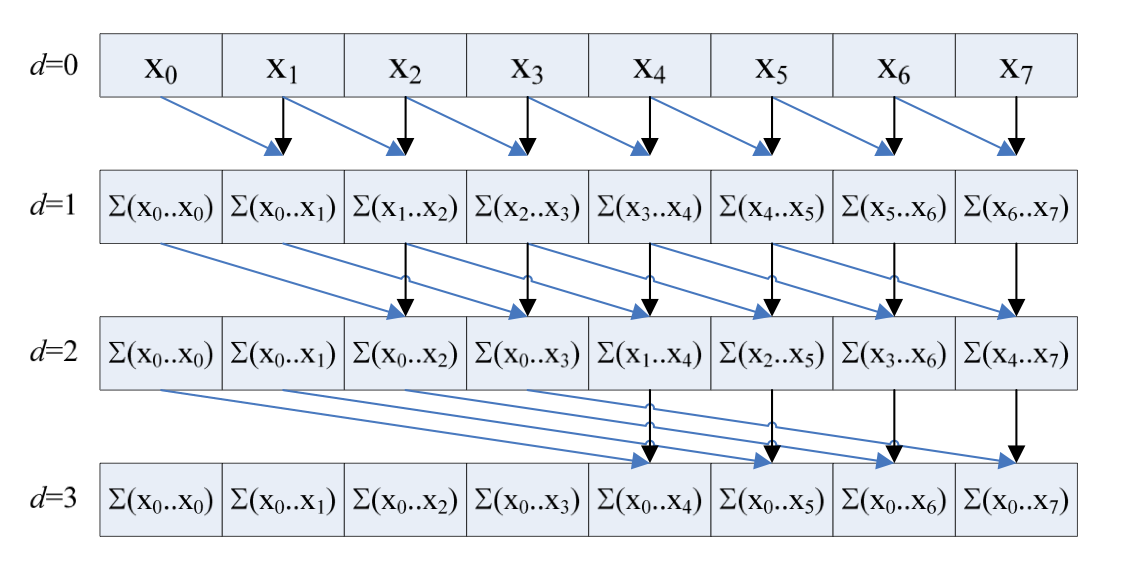
\includegraphics[width=1\textwidth]{res/hillis_and_steele.png} \hfill
\end{center}

\subsubsection{Prefix sum (parallel-prefix)}
Questo tipo di soluzione, compie due passi:
\begin{enumerate}
	\item costruisce un albero in un movimento \textit{bottom-up}, il passo \textit{up}: crea un albero binario, dove la radice ha somma nell'intervallo $[0,n)$ e dove se un nodo ha somma nell'intervallo $[lo, hi)$ e $hi>lo$, allora:
	\begin{itemize}
		\item il figlio sinistro ha somma in $[lo, middle)$;
		\item il figlio destro ha somma in $[middle, hi)$;
		\item una foglia ha somma in $[i, i+1)$, per esempio, $input[i]$.
	\end{itemize}
	Questa è una facile computazione \textit{fork-join}: combina risultati dalla costruzione di un albero binario con tutte le somme degli intervalli (con \textit{work} $O(n)$ e \textit{span} $O(\log{n})$).
	\item attraversa l'albero in un movimento \textit{top-down}, il passo \textit{down}, operando su un valore \textit{fromLeft}:
	\begin{itemize}
		\item la radice da un valore \textit{fromLeft} di $0$;
		\item il nodo prende questo valore \textit{fromLeft} e:
		\begin{itemize}
			\item passa lo stesso al figlio sinistro;
			\item passa $fromLeft$ sommato alla somma del figlio sinistro al figlio destro.
		\end{itemize}
		\item alla foglia in posizione $i$: $output[i] = fromLeft + input[i]$.
	\end{itemize}
	Ancora, sembra una facile computazione \textit{fork-join}: attraversare l'albero costruito nel primo passo e non produrre nessun risultato (con \textit{work} $O(n)$ e \textit{span} $O(\log{n})$).
\end{enumerate}
Ancora, aggiungere un \textit{sequential cutoff} è molto semplice: per la fase \textit{up}, si tratta di una semplice somma, per cui il nodo foglia mantiene la somma di un intervallo; per la fase \textit{down}:
\begin{lstlisting}
output[lo] = fromLeft + input[lo];
for (i=lo+1; i<hi; i++)
	output[i] = output[i-1] + input[i];
\end{lstlisting}

\subsection{Packs: problemi con condizione di verifica}
Dato un array \textit{input}, produrre un array \textit{output} contenente solo gli elementi per cui $f(element)$ è \textit{true}. \\
Esempio:
\begin{center}
	\begin{tabular}{| l | c |}
		\hline
		\textbf{input} & $[17,4,6,8,11,5,13,19,0,24]$ \\
		\textbf{f} & $element > 10$ \\
		\textbf{output} & $[17,11,13,19,24]$ \\
		\hline
	\end{tabular}
\end{center}
E' parallelizzabile? Rintracciare gli elementi è molto semplice (attraverso una mappa), ma metterli al giusto posto sembra complesso:
\begin{enumerate}
	\item Mappa parallela per calcolare un bit-vector per gli elementi per cui $element > 10 = true$;
	\begin{center}
		\begin{tabular}{| l | c |}
			\hline
			\textbf{input} & $[17,4,6,8,11,5,13,19,0,24]$ \\
			\textbf{bits} & $[1,0,0,0,1,0,1,1,0,1]$ \\
			\hline
		\end{tabular}
	\end{center}
	\item prefix-sum parallelo del bit vector:
	\begin{center}
		\begin{tabular}{| l | c |}
			\hline
			\textbf{bitsum} & $[1,1,1,1,2,2,3,4,4,5]$ \\
			\hline
		\end{tabular}
	\end{center}
	\item mappa parallela per produrre l'output:
	\begin{center}
		\begin{tabular}{| l | c |}
			\hline
			\textbf{output} & $[17,11,13,19,24]$ \\
			\hline
		\end{tabular}
		\begin{lstlisting}
output = new array of size bitsum[n-1]
FORALL (i=0; i<input.length; i++) {
	if (bits[i] == 1)
		output[bitsum[i]-1] = input[i];
}
		\end{lstlisting}
	\end{center}
\end{enumerate}

\paragraph{Analisi}
L'algoritmo ha un \textit{work} $O(n)$ e \textit{span} $O(\log{n})$.

\subsection{QuickSort parallelo}
\begin{center}
	\begin{tabular}{| l | l | r |}
		\hline
		\textbf{\#} & \textbf{passo} & \textbf{costo} \\ \hline
		1 & Prendere un elemento \textit{pivot} & $O(1)$ \\
		2 & Partizionare i dati in $A = elem < pivot$, $B = pivot$, $C = elem > pivot$ & $O(n)$ \\
		3 & Ordinare ricorsivamente $A$ e $C$ & $2T(\frac{n}{2})$ \\
		\hline
	\end{tabular}
\end{center}
ha \textit{equazione di ricorrenza} pari a: $R(n) = O(n) + 2\times R(\frac{n}{2})$ \\
Per il \textit{Teorema master}: $O(n\times \log n)$ \\
Il \textit{quicksort} segue tre fasi: scelta dell'elemento \textit{pivot} (che assumeremo sia sempre l'elemento mediano), partizionamento e ordinamento. \\
Per applicare una parallelizzazione seguiremo due soluzioni:
\begin{enumerate}
	\item rendere le chiamate sui due array ricorsive, ottenendo un miglioramento tale: \textit{work} inalterato, \textit{span} pari a $O(n) + 2\times R(\frac{n}{2}) \Rightarrow O(n) + R(\frac{n}{2})$
	\item ottimizzazione dell'operazione di partizionamento, utilizzando il \textit{packing}. Viene lanciato un primo \textit{packing} la cui condizione \`e che gli elementi siano $< pivot$, e poi un secondo per cui la condizione sia che gli elementi siano $> pivot$. \\
	Questo ha \textit{work} $O(n)$ (perch\`e il \textit{work} nei \textit{packing} \`e tale) e \textit{span} $O(n) + R(\frac{n}{2}) \Rightarrow O(\log n) + R(\frac{n}{2})$
\end{enumerate}
Con queste modifiche arriviamo a:
\begin{itemize}
	\item \textit{work}: $O(n)$
	\item \textit{span}: $O(\log^2 n)$
\end{itemize}

\newpage

\subsection{MergeSort parallelo}
\begin{center}
	\begin{tabular}{| l | l | r |}
		\hline
		\textbf{\#} & \textbf{passo} & \textbf{\textit{work} nel \textit{worst-case}} \\ \hline
		1 & Ordinare la metà di sinistra e la metà di destra & $2T(\frac{n}{2})$ \\
		2 & Unire i risultati & $\Theta(n)$ \\
		\hline
	\end{tabular}
\end{center}
Il \textit{MergeSort} generico ha \textit{equazione di ricorrenza}: $R(n) = O(n) + 2\times R(\frac{n}{2})$, che per il \textit{Teorema master} \`e pari a $O(n\times \log n)$.
Le due soluzioni per applicare la parallelizzazione sono le seguenti:
\begin{enumerate}
	\item Utilizzare la parallelizzazione nelle chiamate ricorsive, portando ad un miglioramento tale: $R(n) = O(n) + 2\times R(\frac{n}{2}) \Rightarrow O(n) + R(\frac{n}{2})$
	\item Ottimizzare l'operazione di \textit{merge}: quello che accade \`e che l'array viene splittato in due sottoarray minori o di pari dimensioni o di una differenza di dimensione di 1. In quest'ultimo caso, si sceglie un indice \textit{i} dall'array pi\`u grande perch\`e referenzi l'elemento di mezzo. Nell'array minore, viene scelto un indice \textit{j} tale che, applicata la \textit{ricerca binaria} (di costo $O(\log n)$), alla sua sinistra abbia tutti elementi minori di quello a cui punta l'indice \textit{i} nell'array maggiore. A questo punto vengono lanciate due chiamate ricorsive - parallelamente -, prendendo, nel primo caso, gli array di sinistra, nell'array minore e maggiore, e nel secondo caso quelli di destra. \\
	Poich\`e l'array maggiore sar\`a diviso sempre in subarray di dimensione $n/4$ e poich\`e, nel caso limite, nell'array maggiore, ci troveremo in una situazione tale che il subarray di sinistra avr\`a dimensione $0$ e quello di destra $3/4 \times n$, allora: $R(n) = O(\log n) + R(\frac{n}{4}) + R(\frac{3\times n}{4}) = O(n)$. \\
	Applicando poi la parallelizzazione anche su queste chiamate ricorsive: $R(n) = O(\log n) + R(\frac{3\times n}{4}) = O(\log^2 n)$ \\
	Quindi:
	\begin{itemize}
		\item \textit{work}: $O(n) + 2\times R(\frac{n}{2}) = n \times \log n$
		\item \textit{span}: $O(\log^2 n) + R(\frac{n}{2}) = O(\log^3 n)$
		\item \textit{parallelismo}: $\frac{n}{\log^2 n}$
	\end{itemize}
\end{enumerate}


\newpage

Questo approccio porta a un \textit{work} di:
\begin{center}
	$W(n) = W(\frac{3n}{4}) + W(\frac{n}{4}) + O(\log{n}) = O(n)$
\end{center}
Per lo \textit{span} invece:
\begin{center}
	$S(n) = S(\frac{3n}{4}) + O(\log{n}) = O(\log^{2}n)$
\end{center}
Nel caso sequenziale: $T(n) = 2T(\frac{n}{2}) + \Theta(n) = O(n\times \log{n})$. \\
Quindi, rispetto al sequenziale, il parallelo mantiene lo stesso \textit{work}, ma lo \textit{span} è pari a: $T(n) = 1T(\frac{n}{2}) + \Theta(n) = \Theta(n)$. \\
Utilizzando il parallel merge:
\begin{itemize}
	\item \textit{work}: $T(n) = 2T(\frac{n}{2}) + \Theta(n) = \Theta(n\times \log{n})$;
	\item \textit{span}: $T(n) = 1T(\frac{n}{2}) + \Theta(\log^{2}{n}) = \Theta(\log^{3}{n})$;
	\item \textit{parallelismo}: $O(\frac{n}{\log^{2}{n}})$.
\end{itemize}
Non è ottimale come il \textit{quicksort}, ma garantisce quantomeno un \textit{worst-case}.